%%%%%%%%%%%%%%%%%%%%%%%%%%%%%%%%%%%%
% 	Senior Thesis Template									
%	Saint Vincent College Department of Physics
%	by Zachary Smith
%	May 2022
%	
%	Modifications:
%	
%
%	Instructions:
%
%	Place your .bib file in the same directory as this template 
%	and with the same file name. Typeset this file, followed by the 
%	.bib file, followed by this file twice. 
%
%%%%%%%%%%%%%%%%%%%%%%%%%%%%%%%%%%%%	



\documentclass[longbibliography, 12pt]{article}
\usepackage[paperheight=11in,paperwidth=8.5in,margin =1in]{geometry}
\usepackage{setspace}
\doublespacing
%\pagenumbering{0}
\setlength{\parskip}{1em}
\usepackage[superscript,biblabel]{cite}
\usepackage[english]{babel}
%\usepackage [autostyle, english = american]{csquotes}
%\MakeOuterQuote{"}
% BEGIN bibliography customizations
\usepackage[colorlinks, allcolors=blue]{hyperref}

\bibliographystyle{naturemag}
% END customizations

\usepackage{amsmath}  % needed for \tfrac, \bmatrix, etc.
\usepackage{amsfonts} % needed for bold Greek, Fraktur, and blackboard bold
\usepackage{graphicx} % needed for figures
\usepackage{float}
\usepackage[capitalize]{cleveref}% for referencing figures and tables

\setlength{\parindent}{.5in}
% \graphicspath{ {./images/} }

\newcommand{\subsubsubsection}[1]{\paragraph{#1}\mbox{}\\}
\setcounter{secnumdepth}{4}
\setcounter{tocdepth}{4}

\usepackage{indentfirst}

\begin{document}


	\begin{titlepage}
		\begin{center}
			\textbf{Bose-Hubbard Model \& Machine Learning}
			
			\vspace{5.5cm}
			A thesis submitted to\\ the Department of Physics\\ at Saint Vincent College\\ in partial fulfillment\\ for the degree of\\ Bachelor of Science
			
			\vspace{4.5cm}			
			By\\
			Will Mallah\\
			May 2024

		\end{center}
	\end{titlepage}

\newpage
\begin{abstract}
Although quantum computation is still in the early stages, there are several promising architectures. One of these quantum computing architectures uses Rydberg atoms as qubits. Rydberg atoms, a specific type of Boson, as qubits on a chip, can be modeled by the Bose-Hubbard model. For this reason, we investigated the Bose-Hubbard model. More specifically, we benchmarked code written to simulate this system to determine its accuracy at low scales for extension to higher scale systems. In doing so, it was found that the code operates successfully for the 2 particle, 2 site system. Therefore, we can use the code on higher scale systems with high confidence in the accuracy of its results. Additionally, machine learning models can be implemented to speed up the estimations of desired values within the algorithm.
\end{abstract}

\newpage
\tableofcontents
\newpage
%\setlength{\parindent}{.5in}
		
\section{Introduction}
% Tell the story
%% Talk about what quantum computing is and why it is important
%% Funnel towards the work that I did this past summer
%% Mainly discuss entanglement entropy and why it is important


% What is quantum computing?
%% Rewrite long quote in my owns words
Richard Feynman was the first to conceptualize the idea of using a quantum mechanical system to perform calculations. Not only would this machine be able to perform calculation, but it would also be capable of simulating physical quantum mechanical problems. "Feynman further analyzed that quantum computers can solve quantum mechanical many body problems that are impractical to solve on a classical computer. This is due to the fact that solutions on a classical computer would require exponentially growing time whereas the whole calculations on quantum computer can be done in polynomial time" (Prashant, 7). It was then later discovered by Deutsch, a man whose name is sprinkled through many aspects of quantum computing methods and algorithms, that a general-purpose quantum computer is theoretically possible. Moreover, he "showed that any physical process, in principle could be modelled perfectly by a quantum computer" (Prashant, 7).

The first major application of quantum computation was discovered by Peter Shor, famous for Shor's factorization algorithm: this algorithm was used to successfully factor huge numbers quickly. Since all information on classical computers is kept safe through encryption methods of factoring large prime numbers, this breakthrough gained the attention of many around the world.

% What is entanglement entropy?
One measurement that is of particular interest in quantum computation is entanglement entropy: "Entanglement entropy is a measure of how quantum information is stored in a quantum state" (Hartman, 166).

% Introduction to the work I did over the summer
During the summer of 2023, I worked with Dr. Adrian Del Maestro and his research group at the University of Tennessee Knoxville while attending one of their Research Experience for Undergradutes (REU) programs titled Quantum Alogorithms and Optimization (QAO). During this experience, I worked on benchmarking their algorithm for simulating identical, interacting bosons on a lattice. More specifically, I worked with the small scale (2 particles on 2 sites) in order to confidently extend the simulation to higher scale (larger system sizes). I began my work by studying the theory of the Bose-Hubbard model (\cref*{calculations}). After learning the theory, I began simulating the system using the PIGSFLI algorithm (\cref*{PIGSFLI}). I then compared the results of the PIGSFLI algorithmn to the exact diagonalization (ED) results (\cref*{results}). 


% Finally, I used machine learning to predict the entanglement entropy of the system (\cref*{machine_learning}).

\section{Methods} \label{methods}
The Bose-Hubbard model simulates identical, interacting bosons on lattice. These bosons (particles with whole integer spin) are allowed to live in the same quantum state as other bosons. In the case of the system we looked into, this meant that the bosons were allowed to live on the same site as other bosons. Therefore, an infinite number of bosons could live on the same site at the same time. This system of bosons on a lattice has applications in quantum computation through its use in describing Rydberg atom quantum hardware, where Rydberg atoms are a specific subset of bosons (atoms in this case). To quote Wu in his 2021 paper, "More generally, any atom (moleculeor semiconductor quantum dot) in a state with a highly-excited electron, i.e., with valance electron in a large principal quantum number \textit{n} state of several tens to hundreds or even higher, is regarded as Rydberg atom."\cite{wu_concise_2021}

The following subsection consists of the by-hand exact-diagonalization calculations I preformed during my research experience at the University of Tennessee Knoxville in the summer of 2023. These calculations are split into two main pieces: the first is for first quantization and the second for second quantization. First quantization consists of labeling the system according to the sites where the bosons exist. Second quantization consists of labeling the system according to the individual particles themselves.

\subsection{Bose-Hubbard Calculations} \label{calculations}
\subsubsection{$2^{nd}$ Quantization Von Nuemann Entanglement Entropy Calculation}
To get a better initial feeling for this calculation, we begin with the simpler case: $2^{nd}$ quantization or spatial entanglement. Additionally, systems bigger than 2 particles on 2 sites make by-hand calculations unreadable. Therefore, all following calculations and data analysis only deal with 2 particles on 2 sites for the Bose-Hubbard model. The basis for $2^{nd}$ quantization with 2 particles on 2 sites is as follows:
\begin{equation}
|2 0 \rangle, |1 1 \rangle, |0 2 \rangle,
\end{equation}
\noindent where the left-most number corresponds to the number of bosons on site A and the right-most on site B. The full Hamiltonian for the Bose-Hubbard system is
\begin{equation}
\hat{H} = -J\sum_i{b_i^{\dagger}b_{i+1} + b_{i+1}^{\dagger}b_i} + \frac{U}{2}\sum_i{n_i(n_i - 1)} - \mu\sum_i{n_i},
\label{eq:2}
\end{equation}
\noindent where J is the hopping term, U is the potential energy, and $\mu$ is the chemical potential. $b^{\dagger}$ and $b$ are the creation and annihilation operators, respectively. They act as follows:
\begin{align}
b^{\dagger}|n\rangle &= \sqrt{n+1}\enspace|n+1\rangle \\
b|n\rangle &= \sqrt{n}\enspace|n-1\rangle.
\end{align}
\noindent J, the hopping term, is also denoted as the tunneling term. This term governs how well the particles are able to move between sites. U, the potential energy term, governs the repulsive force between the bosons. This repulsive potential is a result of the bosons approaching each other in close proximity to where their electrons clouds interact, forcing the bosons in opposite directions. 
\noindent The full Hamiltonian can be calculated by calculating the kinetic and potential pieces separately, then simply adding them together. Start by calculating the kinetic energy piece of the full matrix Hamiltonian from \cref{eq:2}. The kinetic energy part of the full hamiltonian above for the 2 particle, 2 site system is
\begin{equation}
\hat{H}_{KE}=-J(b_1^{\dagger}b_2+b_2^{\dagger}b_1).
\end{equation}
\noindent The matrix elements of the kinetic energy part of the Hamiltonian are calculated as follows:
\begin{align*}
\langle{20|H_{KE}|20\rangle} &=0 \\
\langle{11|H_{KE}|20\rangle} &=-\sqrt{2}J \\
\langle{02|H_{KE}|20\rangle} &=0 \\
\langle{20|H_{KE}|11\rangle} &=-\sqrt{2}J \\
\langle{11|H_{KE}|11\rangle} &=0 \\
\langle{02|H_{KE}|11\rangle} &=-\sqrt{2}J \\
\langle{20|H_{KE}|02\rangle} &=0 \\
\langle{11|H_{KE}|02\rangle} &=-\sqrt{2}J \\
\langle{02|H_{KE}|02\rangle} &=0.
\end{align*}
\noindent From these matrix elements, the full kinetic energy piece of the Hamiltonian is written as:
\begin{equation}
\hat{H}_{KE} = \begin{pmatrix} 0 & -\sqrt{2} & 0 \\ -\sqrt{2} & 0 & -\sqrt{2} \\ 0 & -\sqrt{2} & 0 \end{pmatrix}.
\end{equation}
\noindent Next, the potential part of the full Hamiltonian from \cref{eq:2} can be calculated as follows:
\begin{equation}
\hat{H}_{P} = \frac{U}{2}\sum_i{n_i(n_i - 1)} = \frac{U}{2}[n_1(n_1 - 1) + n_2(n_2 - 1)],
\end{equation}
\noindent where $n_i = b_i^{\dagger}b_i$. The elements of the potential part of the Hamiltonian matrix are:
\begin{align*}
\langle{20|H_{P}|20\rangle} &=U \\
\langle{11|H_{P}|20\rangle} &=0 \\
\langle{02|H_{P}|20\rangle} &=0 \\
\langle{20|H_{P}|11\rangle} &=0 \\
\langle{11|H_{P}|11\rangle} &=0 \\
\langle{02|H_{P}|11\rangle} &=0 \\
\langle{20|H_{P}|02\rangle} &=0 \\
\langle{11|H_{P}|02\rangle} &=0 \\
\langle{02|H_{P}|02\rangle} &=U.
\end{align*}
\noindent From these matrix elements, the full potential energy part of the Hamiltonian is written as:
\begin{equation}
\hat{H}_{P} = \begin{pmatrix} U & 0 & 0 \\ 0 & 0 & 0 \\ 0 & 0 & U \end{pmatrix}.
\end{equation}
\noindent The separate kinetic and potential energy pieces of the matrix Hamiltonian can be combined together to make the full matrix as follows:
\begin{equation}
\hat{H} = \begin{pmatrix} U & -\sqrt{2} & 0 \\ -\sqrt{2} & 0 & -\sqrt{2} \\ 0 & -\sqrt{2} & U \end{pmatrix}.
\end{equation}
\noindent Now that we have the full matrix Hamiltonian, we can find the energy states of the system by solving the Schr\"{o}dinger equation. The general form of the Schr\"{o}dinger equation is
\begin{equation}
\hat{H}|\psi\rangle = E|\psi\rangle.
\end{equation}
\noindent Where $E$ is the energy of the system and $|\psi\rangle$ is the wavefunction that describes the system.
\noindent This equation can then be manipulated to look like the following equation:
\begin{equation}
\left( \hat{H}-E\hat{I} \right) |\psi\rangle = 0.
\end{equation}
\noindent Since we are not interested in the solution where $|\psi\rangle=0$, then $\hat{H}-E\hat{I}$ must be zero. This yields the following characteristic equation:
\begin{equation}
\hat{H}-E\hat{I} = 0.
\end{equation}
\noindent This characteristic equation can be solved via expanding the matrix minors and solving the resulting polynomial, where
\begin{equation}
-E^2 + 2UE^2 + 4J^2E - U^2E - 4J^2U = 0.
\label{eq:13}
\end{equation}
\noindent Solving this equation yields 
\begin{align*}
E_1 &= U \\
E_2 &= \frac{1}{2} \left( U - \sqrt{16J^2 + U^2} \right) \\
E_3 &= \frac{1}{2} \left( U + \sqrt{16J^2 + U^2} \right).
\end{align*}
\noindent The solutions to \cref{eq:13} are listed above and are the eigenvalues for the Hamiltonian.  Looking at the three energies listed above, it is obvious that $E_2$ is the ground state energy since it is the lowest of the three. Before the entanglement entropy can be calculated, the density matrix and reduced density matrix must be found. The full density matrix is defined as $\rho = |\psi \rangle \langle \psi|$. The calculation is as follows:
\begin{align}
\hat{\rho} = \left( \alpha |2 0 \rangle + \beta |1 1 \rangle + \gamma |0 2 \rangle \right) \left( \alpha^* \langle 2 0 | + \beta^* \langle 1 1| + \gamma^* \langle 0 2| \right).
\end{align}
\noindent In matrix notation:
\begin{equation}
\hat{\rho} = \begin{bmatrix} \alpha \alpha^* & \alpha \beta^* & \alpha \gamma^* \\ \beta \alpha^* & \beta \beta^* & \beta \gamma^* \\ \gamma \alpha^* & \gamma \beta^* & \gamma \gamma^* \end{bmatrix}.
\end{equation}
\noindent The reduced density matrix is calculated as follows:
\begin{align}
\hat{\rho}_A &= \sum_{n=0}^{2}{{}_B \langle n | \psi \rangle \langle \psi | n \rangle_B} = {}_B \langle 0 | \psi \rangle \langle \psi | 0 \rangle_B + {}_B \langle 1 | \psi \rangle \langle \psi | 1 \rangle_B + {}_B \langle 2 | \psi \rangle \langle \psi | 2 \rangle_B \\
\hat{\rho}_A &=|\alpha|^2 {}_A |2\rangle\langle2|_A + |\beta|^2 {}_A |1\rangle\langle1|_A + |\gamma|^2 {}_A |0\rangle\langle0|_A.
\end{align}
\noindent These elements written in matrix notation are given by:
\begin{equation}
\hat{\rho}_A = \begin{bmatrix} |\alpha|^2 & 0 & 0 \\ 0 & |\beta|^2 & 0 \\ 0 & 0 & |\gamma|^2 \end{bmatrix}
\end{equation}
\noindent Now, we want to calculate the ground state eigenvector. This can be done by substituting our ground state eigenvalue into equation [10] and solving the resulting augmented matrix. This matrix is as follows:
\begin{equation}
\begin{bmatrix} U - \frac{1}{2} \left( U - \sqrt{16J^2 + U^2} \right) & -\sqrt{2}J & 0 \\ -\sqrt{2}J & -\frac{1}{2} \left( U - \sqrt{16J^2 + U^2} \right) & -\sqrt{2}J \\ 0 & -\sqrt{2}J & U - \frac{1}{2} \left( U - \sqrt{16J^2 + U^2} \right) \end{bmatrix} \begin{bmatrix} \alpha \\ \beta \\ \gamma \end{bmatrix} = 0.
\end{equation}
\noindent Solving the above equation provides the solutions for $\alpha$, $\beta$, \& $\gamma$ as follows:
\begin{align*}
\alpha &= \frac{2}{\sqrt{ U'^2 + U' \sqrt{U' + 16} + 16}} = \gamma \\
\beta &= \frac{U' + \sqrt{U' + 16}}{\sqrt{2}\sqrt{U'^2 + U' \sqrt{U' + 16} + 16}},
\end{align*}
\noindent where $U' = \frac{U}{J}$. Finally, the Von Nuemann spatial entanglement entropy is calculated as follows:
\begin{align}
S_1 &= -\text{Tr} \left( \rho_A \ln{\rho_A} \right) = -\text{Tr} \begin{bmatrix} |\alpha|^2 \ln{|\alpha|^2} & 0 & 0 \\ 0 & |\beta|^2 \ln{|\beta|^2} & 0 \\ 0 & 0 & |\gamma|^2 \ln{|\gamma|^2} \end{bmatrix} \\
S_1 &= -\left[ |\alpha|^2 \ln{|\alpha|^2} + |\beta|^2 \ln{|\beta|^2} + |\gamma|^2 \ln{|\gamma|^2} \right]
\end{align}
\noindent This result shows that the Von Neumann entanglement entropy depends only on the elements of the ground state vector of the system: $\alpha$, $\beta$, and $\gamma$.
\subsubsection{$1^{st}$ Quantization Von Nuemann Entanglement Entropy Calculation}
Having obtained the Von Neumann entanglement entropy for $2^{st}$ quantization, we want to run through the same process with $1^{st}$ quantization to obtain the particle entanglement. In the case of $1^{st}$ quantization, we label the particles rather than the sites. The basis for $1^{st}$ quantization is as follows:
\begin{align}
|1_1 2_1 \rangle, |1_1 2_2 \rangle, |1_2 2_1 \rangle, |1_2 2_2 \rangle,
\end{align}
\noindent where the state numbers (i.e., the base numbers) are the particle labels and the subscripts are the site labels (i.e., which site the particle exists on). We begin by calculating the full Hamiltonian, which behaves the same way for $1^{st}$ quantization as it did for $2^{nd}$ quantization:
\begin{equation}
\hat{H} = \begin{bmatrix} \langle 1_1 2_1 | \hat{H} | 1_1 2_1 \rangle & \langle 1_1 2_1 | \hat{H} | 1_1 2_2 \rangle & \langle 1_1 2_1 | \hat{H} | 1_2 2_1 \rangle & \langle 1_1 2_1 | \hat{H} | 1_2 2_2 \rangle \\ \langle 1_1 2_2 | \hat{H} | 1_1 2_1 \rangle & \langle 1_1 2_2 | \hat{H} | 1_1 2_2 \rangle & \langle 1_1 2_2 | \hat{H} | 1_2 2_1 \rangle & \langle 1_1 2_2 | \hat{H} | 1_2 2_2 \rangle \\ \langle 1_2 2_1 | \hat{H} | 1_1 2_1 \rangle & \langle 1_2 2_1 | \hat{H} | 1_1 2_2 \rangle & \langle 1_2 2_1 | \hat{H} | 1_2 2_1 \rangle & \langle 1_2 2_1 | \hat{H} | 1_2 2_2 \rangle \\ \langle 1_2 2_2 | \hat{H} | 1_1 2_1 \rangle & \langle 1_2 2_2 | \hat{H} | 1_1 2_2 \rangle & \langle 1_2 2_2 | \hat{H} | 1_2 2_1 \rangle & \langle 1_2 2_2 | \hat{H} | 1_2 2_2 \rangle \end{bmatrix} 
\end{equation}
\begin{equation}
\hat{H} = \begin{bmatrix} U & -\sqrt{2} & -\sqrt{2} & 0 \\ -\sqrt{2} & 0 & 0 & -\sqrt{2} \\ -\sqrt{2} & 0 & 0 & -\sqrt{2} \\ 0 & -\sqrt{2} & -\sqrt{2} & U \end{bmatrix}.
\end{equation}
\noindent The full density matrix is then given by $|\psi \rangle \langle \psi|$, where $\psi$, the ground state, is given by:
\begin{equation*}
\psi = \alpha |1_1 2_1 \rangle + \frac{\beta}{\sqrt{2}} \left( |1_1 2_2 \rangle + |1_2 2_1 \rangle \right) + \gamma |1_2 2_2 \rangle,
\end{equation*}
\iffalse
\begin{equation}
\hat{\rho} = \begin{bmatrix} \langle 1_1 2_1 | \hat{\rho} | 1_1 2_1 \rangle & \langle 1_1 2_1 | \hat{\rho} | 1_1 2_2 \rangle & \langle 1_1 2_1 | \hat{\rho} | 1_2 2_1 \rangle & \langle 1_1 2_1 | \hat{\rho} | 1_2 2_2 \rangle \\ \langle 1_1 2_2 | \hat{\rho} | 1_1 2_1 \rangle & \langle 1_1 2_2 | \hat{\rho} | 1_1 2_2 \rangle & \langle 1_1 2_2 | \hat{\rho} | 1_2 2_1 \rangle & \langle 1_1 2_2 | \hat{\rho} | 1_2 2_2 \rangle \\ \langle 1_2 2_1 | \hat{\rho} | 1_1 2_1 \rangle & \langle 1_2 2_1 | \hat{\rho} | 1_1 2_2 \rangle & \langle 1_2 2_1 | \hat{\rho} | 1_2 2_1 \rangle & \langle 1_2 2_1 | \hat{\rho} | 1_2 2_2 \rangle \\ \langle 1_2 2_2 | \hat{\rho} | 1_1 2_1 \rangle & \langle 1_2 2_2 | \hat{\rho} | 1_1 2_2 \rangle & \langle 1_2 2_2 | \hat{\rho} | 1_2 2_1 \rangle & \langle 1_2 2_2 | \hat{\rho} | 1_2 2_2 \rangle \end{bmatrix} 
\end{equation}
\fi
\noindent where $\alpha$, $\beta$, and $\gamma$ are the elements of the ground state vector of the system. The full density matrix is
\begin{equation}
\hat{\rho} = \begin{bmatrix} |\alpha|^2 & \frac{\alpha \beta^*}{\sqrt{2}} & \frac{\alpha \beta^*}{\sqrt{2}} & \alpha \gamma^* \\ \frac{\beta \alpha^*}{\sqrt{2}} & \frac{|\beta|^2}{2} & \frac{|\beta|^2}{2} & \frac{\beta \gamma^*}{\sqrt{2}} \\ \frac{\beta \alpha^*}{\sqrt{2}} & \frac{|\beta|^2}{2} & \frac{|\beta|^2}{2} & \frac{\beta \gamma^*}{\sqrt{2}} \\ \gamma \alpha^* & \frac{\gamma \beta^*}{\sqrt{2}} & \frac{\gamma \beta^*}{\sqrt{2}} & |\gamma|^2 \end{bmatrix}.
\end{equation}
\noindent We then needed to calculate the reduced density matrix, which is given by tracing out the degrees of freedom of the second particle. The reduced density matrix is as follows:
\begin{align}
\hat{\rho}_A &= \sum_{n=1}^{2} {}_B \langle n|\psi \rangle \langle \psi|n \rangle_B = {}_B\langle 2_1|\psi \rangle \langle \psi|2_1 \rangle_B + {}_B\langle 2_2|\psi \rangle \langle \psi|2_2 \rangle_B.
\end{align}
The only surviving terms from the above calculation are
\begin{align*}
\hat{\rho}_A &= \left( |\alpha|^2 + \frac{|\beta|^2}{2} \right) {}_A |1_1 \rangle \langle 1_1|_A
+ \left( \frac{\alpha \beta^* + \beta \gamma^*}{\sqrt{2}} \right) {}_A |1_1 \rangle \langle 1_2|_A \\
&+ \left( \frac{\beta \alpha^*+ \gamma \beta^*}{\sqrt{2}} \right) {}_A |1_2 \rangle \langle 1_1|
+ \left( \frac{|\beta|^2}{2} + |\gamma|^2 \right) {}_A |1_2 \rangle \langle 1_2|_A.
\end{align*}
\begin{equation}
\hat{\rho}_A = \begin{bmatrix} {}_A \langle 1_1 | \hat{\rho_A} | 1_1 \rangle & {}_A \langle 1_1 | \hat{\rho_A} | 1_2 \rangle \\ {}_A \langle 1_2 | \hat{\rho_A} | 1_1 \rangle & {}_A \langle 1_2 | \hat{\rho_A} | 1_2 \rangle \end{bmatrix} = \begin{bmatrix} |\alpha|^2 + \frac{|\beta|^2}{2} & \frac{\alpha \beta^* + \beta \gamma^*}{\sqrt{2}} \\ \frac{\beta \alpha^* + \gamma \beta^*}{\sqrt{2}} & \frac{|\beta|^2}{2} + |\gamma|^2 \end{bmatrix} \\
\hat{\rho}_A = \begin{bmatrix} \frac{1}{2} & \sqrt{2} \alpha \beta \\ \sqrt{2} \alpha \beta & \frac{1}{2} \end{bmatrix}.
\end{equation}
\noindent To get the Von Nuemann entanglement entropy, the eigenvalues of the above matrix are needed. To obtain these eigenvalues, the following equation must be solved:
\begin{equation}
\hat{\rho}_A - \lambda \hat{I} = 0, \\
\end{equation}
\noindent where $\lambda$ is the eigenvalue we are solving for. In matrix form, this becomes:
\begin{equation}
\begin{bmatrix} \frac{1}{2} - \lambda & \sqrt{2} \alpha \beta \\ \sqrt{2} \alpha \beta & \frac{1}{2} - \lambda \end{bmatrix} = 0.
\end{equation}
\noindent Taking the determinant of this equation yields the characteristic equation:
\begin{align}
\lambda^2 - \lambda - 2 \alpha^2 + 4 \alpha^4 + \frac{1}{4} &= 0.
\end{align}
\noindent The eigenvalues can then be calculated using the quadratic equation:
\begin{align}
\lambda_{\pm} &= \frac{1 \pm \sqrt{1^2 - 4 \left( 1 \right) \left( -2 \alpha^2 + 4 \alpha^4 + \frac{1}{4} \right) }}{2} = \frac{1 \pm 2 \alpha \sqrt{2 - 4 \alpha^2}}{2}.
\label{eq:lambda_pm}
\end{align}
\noindent The Von Nuemann particle entanglement entropy is then calculated as follows:
\begin{align}
S_1 &= -\text{Tr} \left( \rho_A \ln{\rho_A} \right) = -\text{Tr} \begin{bmatrix} \lambda_+ & 0 \\ 0 & \lambda_- \end{bmatrix} \begin{bmatrix} \ln{\lambda_+} & 0 \\ 0 & \ln{\lambda_-} \end{bmatrix} \\
S_1 &= -\lambda_+ \ln{\lambda_+} - \lambda_- \ln{\lambda_-}
\end{align}
\noindent where $\lambda_+$ and $\lambda_-$ are defined by \cref*{eq:lambda_pm}. Similar to the Von Neumann entanglement entropy calculation for $2^{nd}$ quantization, the entanglement entropy for $1^{st}$ quantization also depends only on the elements of the ground state vector for the system.

\section{Discussion}

\begin{figure}[h]
\centering
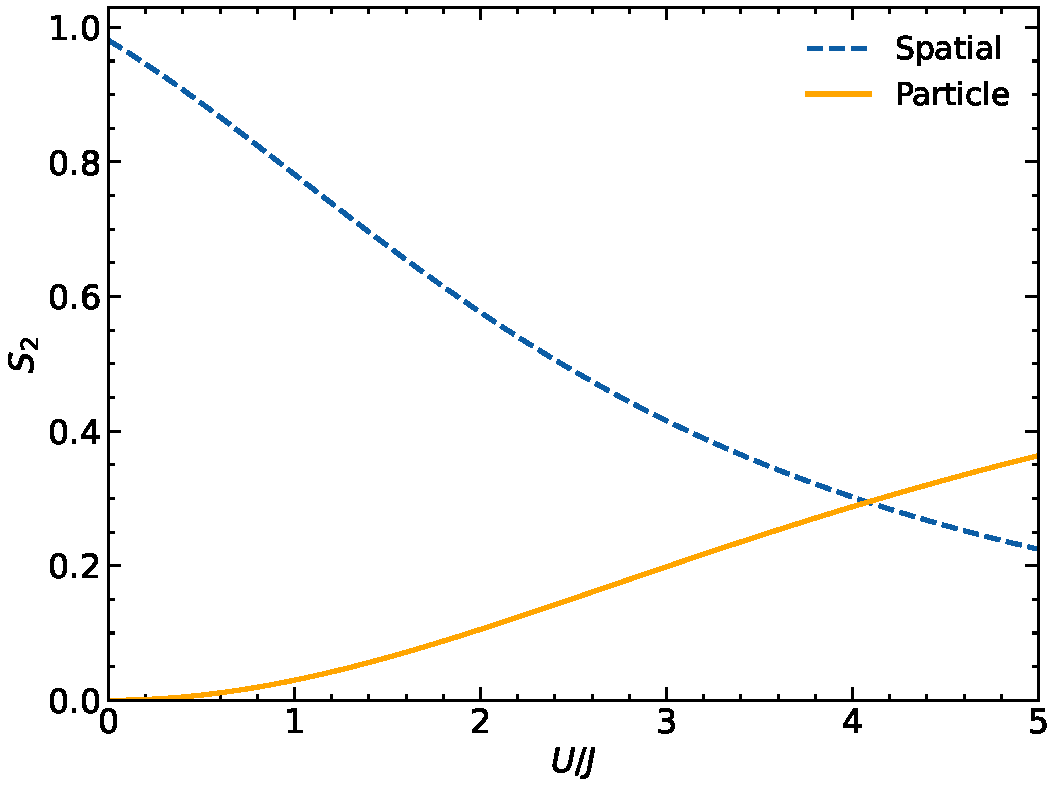
\includegraphics[scale=0.5]{../figures/ed_renyi.pdf}
\caption{The figure above is a graph of the Renyi entanglement entropy for both spatial and particle bipartitions versus the ratio of the interaction term to the hopping term.}
\end{figure}

\subsection{PIGSFLI Algorithm}

A Monte Carlo simulation is a stochastic (random) method of integration, which allows for accurate estimations of desired values. Monte Carlo is necessary for situations where exact calculations are too computationally expensive, such as in the exact diagonalization of the reduced density matrix for high particle/site number Bose Hubbard systems. The size of the Hilbert space is calculated by \cref{eq:36} and shown by \cref{fig:hilbert_space_size}:

\begin{equation}
D = \frac{\left(N+L-1\right)!}{\left(N\right)!\left(L-1\right)!}
\label{eq:36}
\end{equation}

\begin{figure}[h]
\centering
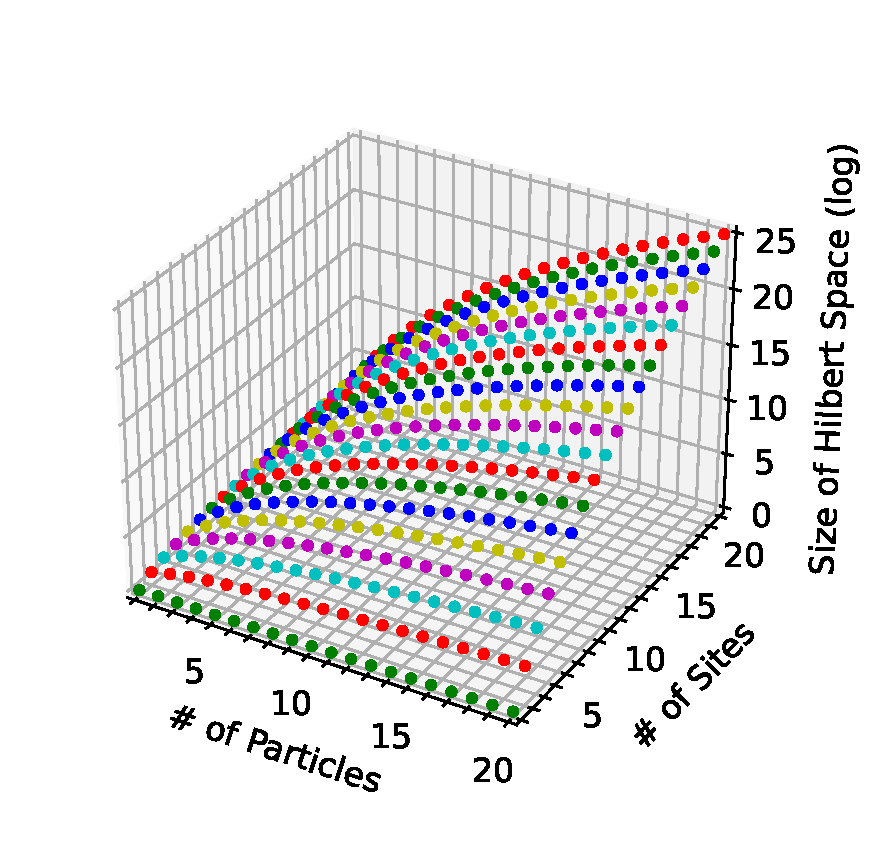
\includegraphics[scale=0.5]{../figures/hilbert_space_size.pdf}
\caption{The figure above shows the size of the Hilbert space as a function of number of sites and particles. This 3-dimensional plot for the number of combinations in the Hilbert space goes up to $20$ sites and $20$ particles.}
\label{fig:hilbert_space_size}
\end{figure}


\begin{figure}
\centering
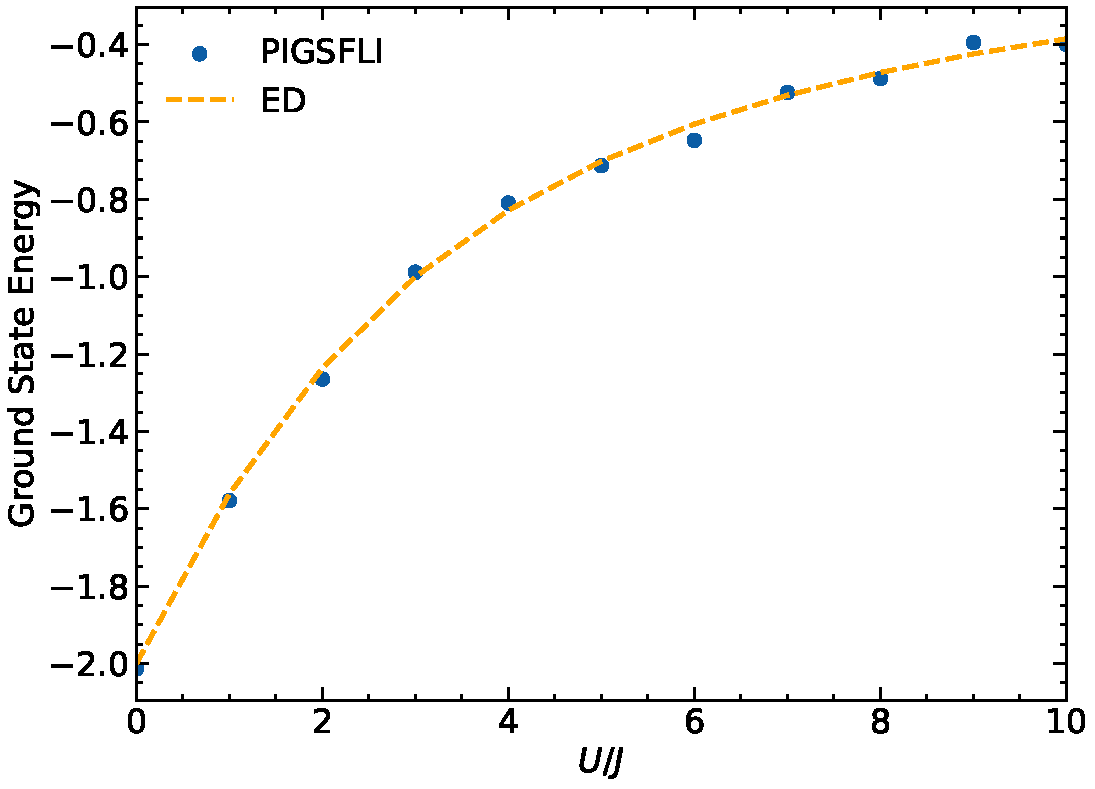
\includegraphics[scale=0.5]{../figures/total_energy.pdf}
\caption{A plot of the ground state energy versus the ratio between U, the potential term, and J, the hopping term for both exact diagonalization and PIGSFLI algorithm. From this plot, the PIGSFLI reults match very well to our ED calculation.}
\label{fig:total_energy}
\end{figure}

\begin{figure}
\centering
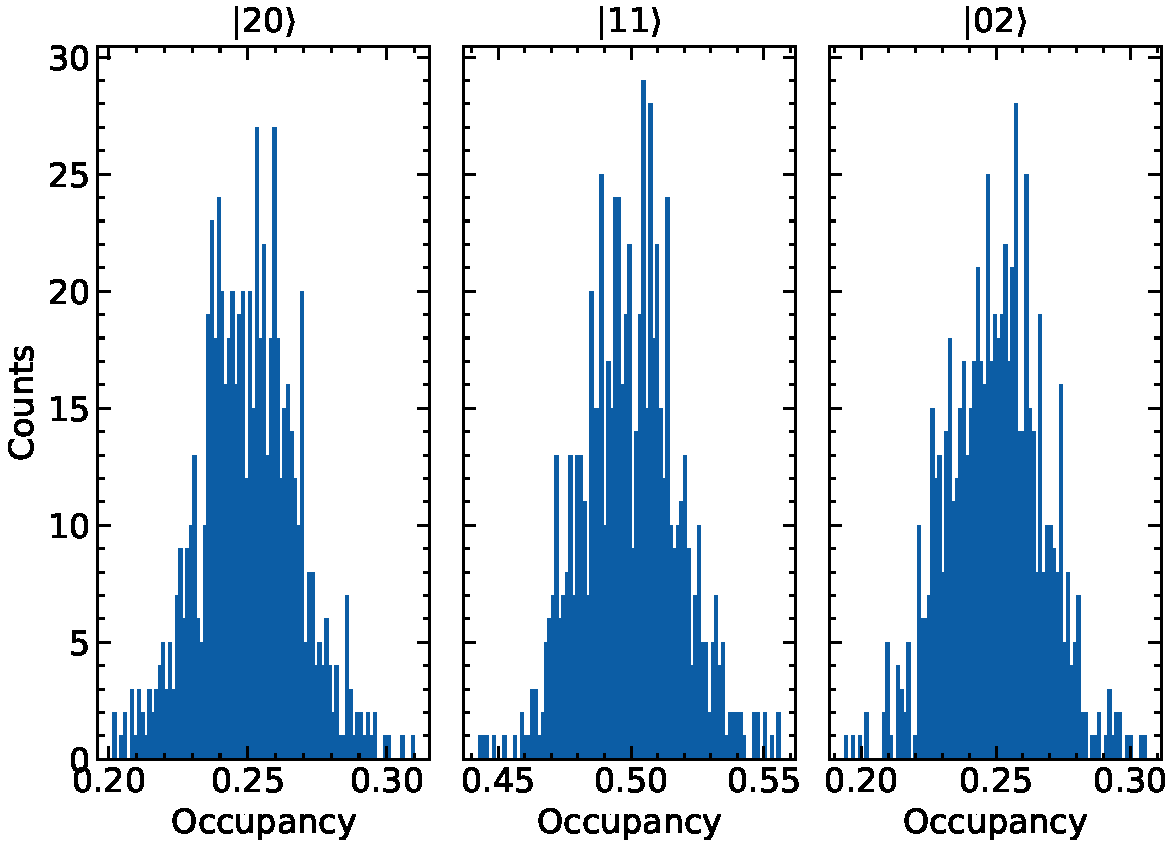
\includegraphics[scale=0.5]{../figures/sep_occ_hist_U_0.0001.pdf}
\caption{The figure above shows the histogram of the occupation number for the particle bipartition as a function of the ratio of the interaction term to the hopping term. This graph specifically shows the case where the interaction term is $10$ times the hopping term.}
\label{fig:sep_occ_hist_U_0.0001}
\end{figure}

\begin{figure}
\centering
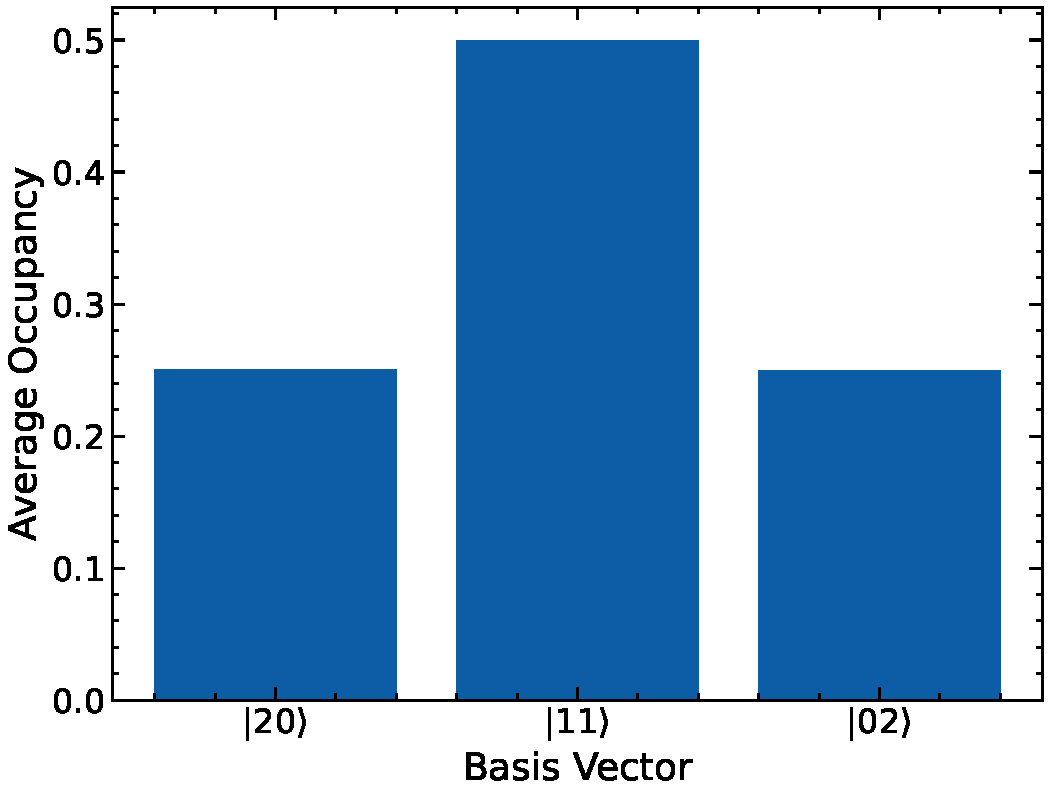
\includegraphics[scale=0.5]{../figures/spatial_avg_occ_U_0.0001.pdf}
\caption{The figure above shows the average occupation number for the spatial bipartition as a function of the ratio of the interaction term to the hopping term. This graph specifically shows the case where the interaction term is $10$ times the hopping term.}
\label{fig:spatial_avg_occ_U_0.0001}
\end{figure}

\begin{figure}
\centering
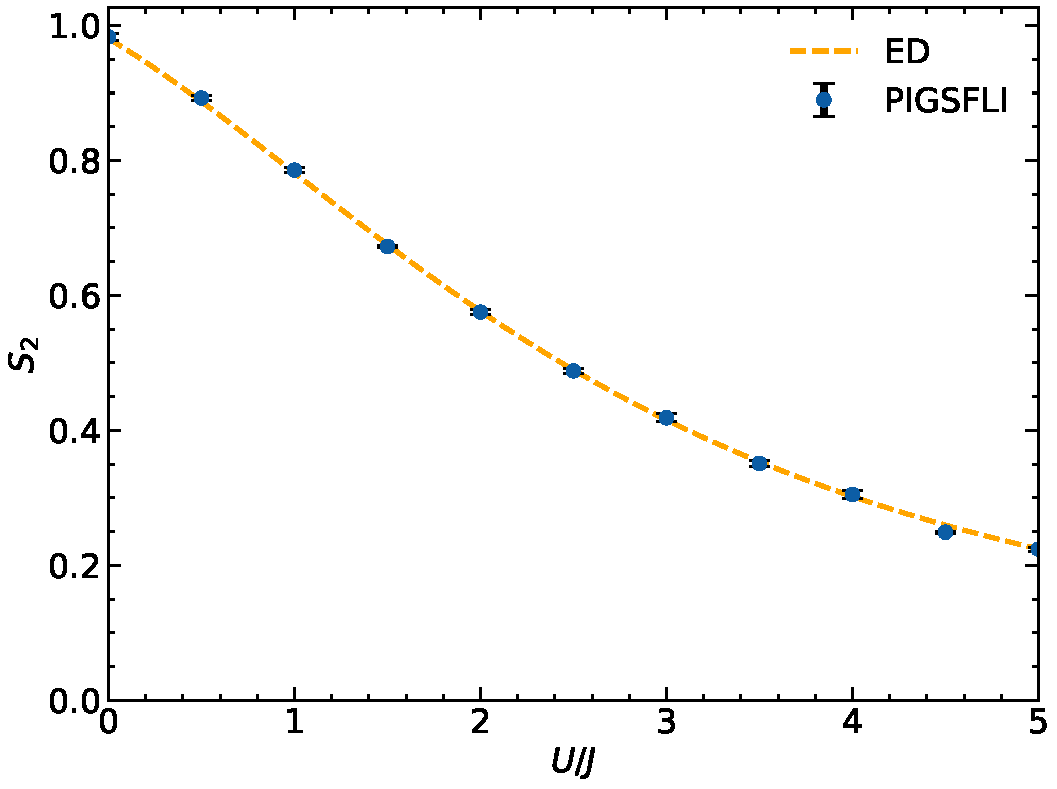
\includegraphics[scale=0.5]{../figures/renyi_spatial.pdf}
\caption{The second Rényi spatial entanglement entropy as a function of U/J for both exact diagonalization (ED) and PIGSFLI. This plot shows excellent agreement between the PIGSFLI estimation and that of our ED calculation, showing that PIGSFLI is a viable option for computation on much larger system sizes.}
\label{fig:renyi_spatial}
\end{figure}


\newpage
\bibliography{main.bib}% For BibTex

% \newpage
% \AtEndDocument{\section{Appendix A: More interesting details}

% Here are details in an Appendix.

% }

\end{document}